\documentclass[a4paper,12pt]{article}

%-----------------------------------------------
% Document variables

\newcommand{\myTitle}{Swing-up of a triple arm inverted pendulum\xspace}
\newcommand{\mySubtitle}{Master semester project\xspace}
\newcommand{\myDegree}{Master of science of Mechanical engineering\xspace}
\newcommand{\myName}{Frederic Nguyen\xspace}
\newcommand{\myProf}{Philipe Müllhaupt\xspace}
\newcommand{\mySupervisor}{Ehsan Sarshari\xspace}
\newcommand{\myFaculty}{Laboratoire d'automatique\xspace}
\newcommand{\myDepartment}{Mechanical engineering\xspace}
\newcommand{\myUni}{Ecole polytechnique fédérale de Lausanne\xspace}
\newcommand{\myLocation}{Lausanne\xspace}
\newcommand{\myTime}{December 2016\xspace}
\newcommand{\myVersion}{version 1.0\xspace}



%-------------------------------------------
%	CHARACTER ENCODING
%-------------------------------------------
\usepackage[utf8]{inputenc}

%-------------------------------------------
%	USEFUL COMMANDS
%-------------------------------------------

%-------------------------------------------
%	PACKAGES
%-------------------------------------------
\usepackage[english]{babel}

\usepackage{sectsty}

\usepackage{titlesec}

\usepackage{mathtools}

%------------------------------------------------
\usepackage{array,multirow}
\usepackage{booktabs}
%------------------------------------------------
\usepackage[dvipsnames]{xcolor}
%------------------------------------------------
\usepackage{textcomp}
\usepackage{enumitem}
\usepackage[load-configurations = abbreviations]{siunitx}
% \sisetup{locale = FR, range-phrase={ \`{a} }, list-final-separator={ et }, list-pair-separator={ et }, detect-all}
\usepackage{float,sidecap}
%------------------------------------------------
\usepackage[tracking]{microtype}
% \usepackage{mathptmx} % Corpus font
% \usepackage{newtxtext}
% \usepackage{newtxmath}
\usepackage{fourier}
\DeclareMathAlphabet{\mathcal}{OMS}{cmsy}{m}{n}
\usepackage[condensed]{roboto}
%\renewcommand{\sfdefault}{fvs} % Lato for 1st page and section titles fla
%\linespread{1.025}
%------------------------------------------------
\usepackage{import}
%\usepackage[final]{pdfpages}
\usepackage{graphicx}

%------------------------------------------------
\usepackage[a4paper]{geometry}
\usepackage[format=hang,font=small,labelfont={sf,bf},labelsep=endash]{caption}
\geometry{top=2.54cm, bottom=2.5cm, left=2.54cm , right=2.54cm}
%------------------------------------------------
\usepackage[T1]{fontenc}
%------------------------------------------------
\usepackage{fancyhdr}
\pagestyle{fancy}
\renewcommand{\sectionmark}[1]{\markright{\MakeUppercase{\thesection.\ #1}}}

\fancyhf{}
\fancyhead[LE,RO]{}
\fancyhead[RE,LO]{\rightmark}
\fancyfoot[CE,CO]{}
\fancyfoot[LE,RO]{\thepage}

%------------------------------------------------
\setlist{noitemsep}


%------------------------------------------------
\graphicspath{{illustrations/}{../illustrations/}}
%\allsectionsfont{\sffamily}
%\frenchbsetup{og = «, fg = »}
%\urlstyle{sf}
\usepackage{xcolor} % Required for specifying colors by name
\definecolor{ocre}{RGB}{52,177,201} % Define the orange color used for highlighting throughout the book
\definecolor{blackout}{RGB}{0,0,0}

\usepackage{titlesec}
% use \llap if you want to align text section with left textwidth
\makeatletter
\renewcommand{\@seccntformat}[1]{\textcolor{black!55}{\csname the#1\endcsname}\hspace{0.5em}}                    
\renewcommand{\section}{\@startsection{section}{1}{\z@}
{-2.5ex}
{0.5ex }
{\normalfont\Large\sffamily\bfseries}}

\renewcommand{\subsection}{\@startsection {subsection}{2}{\z@}
{-1.5ex}
{0.5ex}
{\large\sffamily\bfseries}}

\renewcommand{\subsubsection}{\@startsection {subsubsection}{3}{\z@}
{-2ex \@plus -0.1ex \@minus -.2ex}
{.2ex \@plus.2ex }
{\sffamily\bfseries}}

\renewcommand\paragraph{\@startsection{paragraph}{4}{\z@}
{-2ex \@plus-.2ex \@minus .2ex}
{.1ex}
{\sffamily\bfseries\itshape}}
\makeatother

% \titleformat{\section}
% {\sffamily\large\bfseries\uppercase}{\thesection}{.5em}{}

% \titlespacing{\section}{0pt}{1em}{0.5em}

\usepackage{titletoc} % Required for manipulating the table of contents
\contentsmargin{0cm} % Removes the default margin
% Chapter text styling
%\titlecontents{chapter}[1.25cm] % Indentation
%{\addvspace{15pt}\large\sffamily\bfseries} % Spacing and font options for chapters
%{\color{ocre!60}\contentslabel[\Large\thecontentslabel]{1.25cm}\color{ocre}} % Chapter number
%{}  
%{\color{ocre!60}\normalsize\sffamily\bfseries\;\titlerule*[.5pc]{.}\;\thecontentspage} % Page number

% Section text styling
%\titlecontents{section}[1.25cm] % Indentation
%{\addvspace{5pt}\sffamily\bfseries} % Spacing and font options for sections
%{\contentslabel[\thecontentslabel]{1.25cm}} % Section number
%{}
%{\sffamily\hfill\color{black}\thecontentspage} % Page number
%[]
\titlecontents{section}[0.5cm] % Indentation
{\addvspace{6pt}\large\sffamily\bfseries} % Spacing and font options for chapters
{\color{black!50}\contentslabel[\Large\thecontentslabel]{0.7cm}\color{black}} % Section number
{}  
{\color{black!50}\normalsize\sffamily\bfseries\;\titlerule*[.5pc]{}\;\thecontentspage} % Page number

% Subsection text styling
%\titlecontents{subsection}[1.25cm] % Indentation
%{\addvspace{5pt}\sffamily\small} % Spacing and font options for subsections
%{\contentslabel[\thecontentslabel]{1.25cm}} % Subsection number
%{}
%{\sffamily\;\titlerule*[.5pc]{.}\;\thecontentspage} % Page number
%[]

\titlecontents{subsection}[1.4cm] % Indentation
{\addvspace{3pt}\sffamily\bfseries} % Spacing and font options for subsections
{\color{black!50}\contentslabel[\thecontentslabel]{0.8cm}\color{black}} % Section number
{}
{\sffamily\bfseries\color{black!50}\;\titlerule*[.6pc]{.}\;\thecontentspage} % Page number
[]

% Subsubsection text styling
\titlecontents{subsubsection}[2.5cm] % Indentation
{\addvspace{1pt}\sffamily\small\bfseries} % Spacing and font options for subsubsections
{\color{black!50}\contentslabel[\thecontentslabel]{1cm}\color{black}} % Subsubsection number
{}
{\sffamily\bfseries\color{black!50}\;\titlerule*[.6pc]{.}\;\thecontentspage} % Page number
[]

%-----------------------------------------------
% DOCUMENT BEGINS HERE
%-----------------------------------------------
\begin{document}
\renewcommand{\headheight}{14.5pt}
\renewcommand{\tablename}{Table}
\renewcommand{\figurename}{Figure}

% Title page
\hypersetup{pageanchor=false}
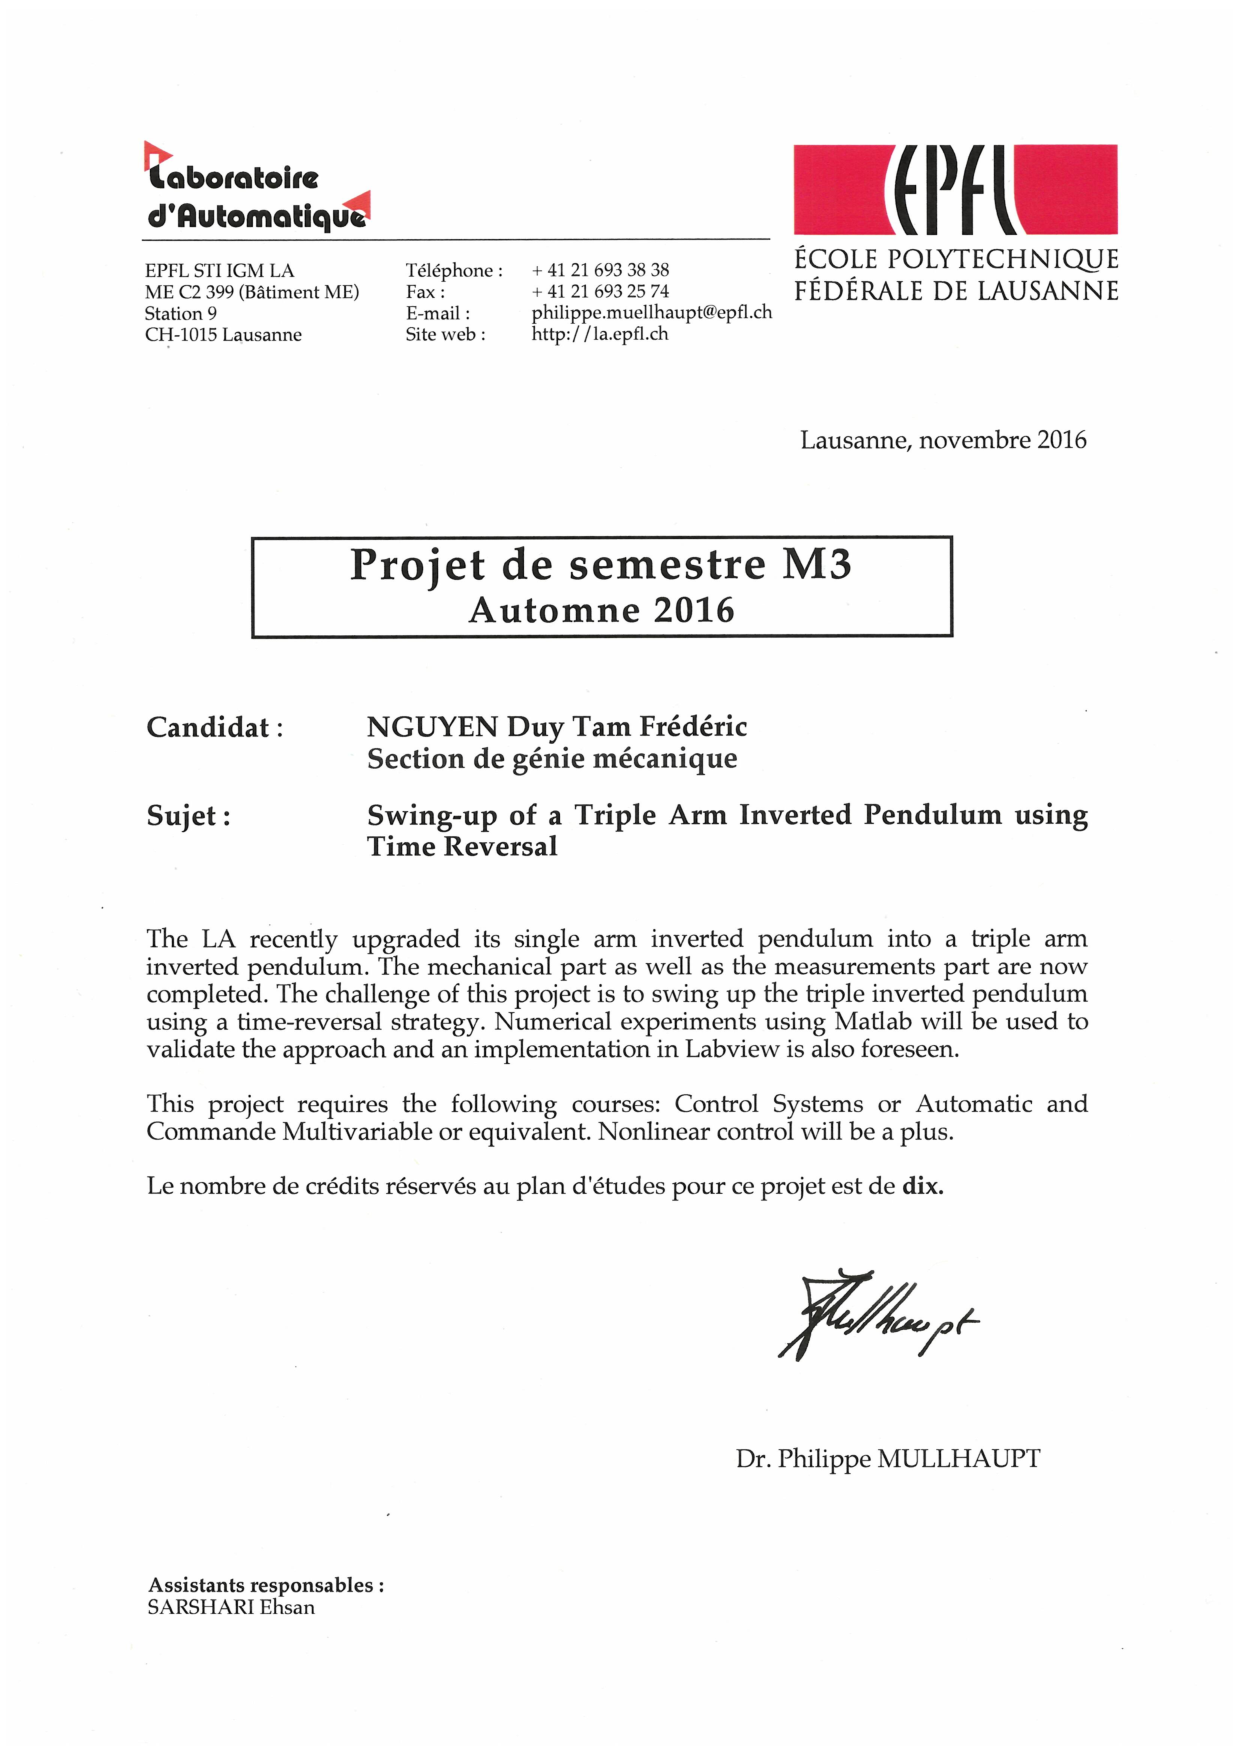
\includepdf{DNguyen.pdf}
% \begin{titlepage}

\newcommand{\HRule}{\rule{\linewidth}{0.5mm}} % Defines a new command for the horizontal lines, change thickness here


\center % Center everything on the page
%----------------------------------------------------------------------------------------
%	LOGO SECTION
%----------------------------------------------------------------------------------------

\includegraphics[width=5cm]{logo_automatique}
\hfill

\includegraphics[width=5cm]{epfl}\\[4.5cm]

%----------------------------------------------------------------------------------------
%	HEADING SECTIONS
%----------------------------------------------------------------------------------------
%\normalfont\fontsize{26}{26}\sffamily\selectfont
%\textbf{Clustering the interstellar medium}\\
%{\LARGE Data Mining and Machine Learning in Astronomy}
%\textsc{ }\\[6cm]


%----------------------------------------------------------------------------------------
%	TITLE SECTION
%----------------------------------------------------------------------------------------

\HRule \\[0.2cm]
\sffamily
{\LARGE\bfseries \uppercase{Swing-up of a triple arm inverted pendulum}} \\[0.05cm]
{\Large\bfseries Master Semester Project}
\HRule \\[0.5cm]
 
%----------------------------------------------------------------------------------------
%	AUTHOR SECTION
%----------------------------------------------------------------------------------------

{\Large Laboratoire d'automatique}\\[0.1cm] % Name of your university/college
{\large Mechanical Engineering Faculty}\\[4.5cm] % Major heading such as course name

\begin{minipage}{0.45\textwidth}
    \begin{flushleft}
        \textbf{Author:}\\
        Frédéric NGUYEN
    \end{flushleft}
\end{minipage}
~
\begin{minipage}{0.45\textwidth}
    \begin{flushright}
        \textbf{Professor:} \\
        Dr. Philipe MÜLLHAUPT\\
        \textbf{Supervisor:}\\
        Ehsan SARSHARI
    \end{flushright}
\end{minipage}\\[2cm]

% If you don't want a supervisor, uncomment the two lines below and remove the section above
%\Large \emph{Author:}\\
%John \textsc{Smith}\\[3cm] % Your name

%----------------------------------------------------------------------------------------
%	DATE SECTION
%----------------------------------------------------------------------------------------
\vfill
{Lausanne, le 28 Décembre 2016}\\[1.5cm] % Date, change the \today to a set date if you want to be precise


 
%----------------------------------------------------------------------------------------

\vfill % Fill the rest of the page with whitespace

\end{titlepage}
\hypersetup{pageanchor=true}
\newpage


%---------------------------------------------------------------
%	ABSTRACT
%---------------------------------------------------------------
\pagenumbering{roman}
\begin{abstract}
In this report, the subject of the swing-up control of a triple arm inverted pendulum is approached. The swing-up strategy uses a time-reversal strategy. It is based on reproducing the reversed behaviour of a known desired trajectories of a falling triple pendulum. The focuses handled are the mathematical modeling of the triple pendulum, the elaboration of a controller for tracking a planned motion and the simulation of the swing-up phase by using the described strategy in MATLAB environment.

\noindent
\textbf{Keywords: }Triple pendulum, swing-up, time-reversal strategy, LQR controller
\end{abstract}
\newpage
% Summary
\thispagestyle{empty}
\tableofcontents
\newpage

\pagenumbering{arabic}



%---------------------------------------------------------------
%	INTRODUCTION
%---------------------------------------------------------------
\section{Introduction}\label{sec:intro} %ABSTRACT
The triple arm inverted pendulum is a typical problem in the control system field. Since it has less actuators than degrees of freedom, this under-actuated system constitutes an excellent test bench for testing and evaluating many types of controllers. Moreover its non-linearity, a dynamics behaviour governed by coupled ordinary differential equations make the regulation task complicated.

When approaching the regulation of an inverted pendulum, there is a need to separate it in two tasks: the stabilization and the swing-up. Each of these tasks have seen numerous contributions and these contributions reflects the diversity of control techniques. For example the stabilization task is handled with a state feedback design by \citet{Medrano1997} or with a controller based on the LQR method designed by \citet{Gupta2014}. The swing-up task has also seen noticeable improvements provided by the papers from \citet{Astrom2000287} and \citet{Gluck2013801}.

This study aims to evaluate the feasibility of the swing-up strategy for the triple arm inverted pendulum. It will begin with a mathematical modeling of the system. Then some concepts such as controllability of a system and design of LQR controllers are discussed in this report. Finally, simulations from the MATLAB environment of the swing-up phase are presented. The project is restricted to pure simulations studies.

% The swing-up of a triple arm inverted pendulum is presented. The main focus of this semester project is to simulate a strategy for the swing-up of the pendulum. The goal of this project is to provide a solution for the swing-up of a triple arm inverted pendulum.
% restricted to pure simulations studies.
% This project is based on the use of symbolic math toolbox and numeric simulations on MATLAB

%---------------------------------------------------------------
%	PRINCIPLE OF THE SWING-UP STRATEGY
%---------------------------------------------------------------
\begin{figure}[ht]
	\centering
	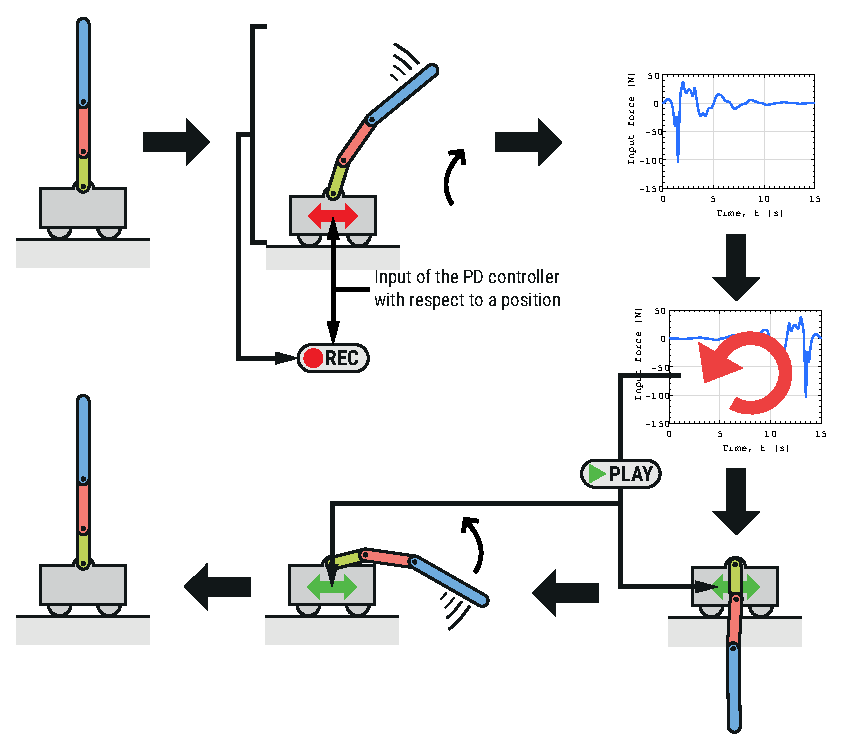
\includegraphics[width=1\textwidth]{principle_swingup}
	\caption{Principle of the swing-up strategy}
	\label{fig:swingup_strategy}
\end{figure}
\section{Principle of the swing-up strategy}
The main focus of this project is the swing-up phase of the pendulum. This phase consists in leading the cart of the triple pendulum from the stable equilibrium to an unstable equilibrium where all the arms are in the upright position. 

The principle is resumed in \autoref{fig:swingup_strategy}. The first step (phases 1 and 2) is to let fall the triple pendulum from its unstable equilibrium to its stable equilibrium. A PD controller which applies to the cart acts as a damper. Meanwhile the falling of the three links, their angles and angular velocities are recorded (phases 2 and 3) as well as the position and velocity of the cart, and the input of the PD controller. The recording is stopped after a certain time or until the triple pendulum is stabilized. Then the logged input PD controller is reversed (phase 3) and implemented to the triple pendulum for the swing-up. The system have the same behaviour recorded previously but in the reversed time or way (phase 6). 

%---------------------------------------------------------------
%	MODELING OF THE TRIPLE PENDULUM
%---------------------------------------------------------------
\section{Modeling of the triple pendulum}
For the purpose of this project, it is required to develop the equations of motion of the triple pendulum system. A \emph{Lagrangian approach} is used for the modeling of the triple pendulum. The obtained model is linearized around operating configuration such as the down and up configuration. In the following pages, vector and matrix quantities are identified in bold characters.

\subsection{Description of the triple pendulum}
The pendulum consists in three links mounted on a cart. The cart is driven on a rail track. It is the only actuated part of the system. The other parts are free to move in their degree of freedom. For each link, a length and a mass is defined. The links are supposed to be made of homogeneous material so the gravity center for each one are on the geometrical middle of each bars. The viscous frictions in the bears of the cart and the links are neglected for the modeling of the triple pendulum.

A schematic representation of the system is showed in \autoref{fig:schematic_system}. The dispositions of the positions and angles, and the coordinate system are showed in \autoref{fig:schematic_system}; they will be used for the modeling of the pendulum.
\begin{figure}[ht]
	\centering
	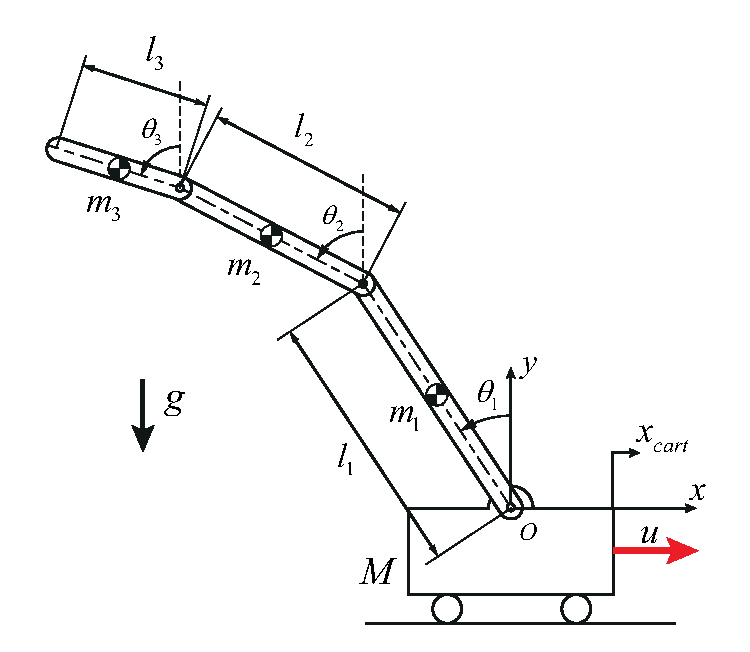
\includegraphics[width=11cm]{illustrations/schematic_system.eps}
	\caption{Triple arm inverted pendulum with assumed coordinate systems, dimensions and angles}
	\label{fig:schematic_system}
\end{figure}

Since the triple pendulum is a 4-degree-of-freedom system, there are four generalized coordinates which are defined for this pendulum. The first one is the position of the cart $x_{cart}$ with respect to a reference. The last three generalized coordinates are the angles ($\theta_1$, $\theta_2$, $\theta_3$) of links at the joints. Their zero value are when the bars are in up position and they increase their values when turning counterclockwise. The assignment of each degree of freedom to a generalized coordinate is according to the following:
\[
	x_{cart}\to q_1, \qquad \theta_1\to q_2, \qquad \theta_2\to q_3, \qquad \theta_3\to q_4
\]

The parameters of the system are given values in \autoref{tab:parameters_system} and will be used for every numerical simulation of the triple pendulum.
\begin{table}[H]
	\centering
	\caption{Parameters for the following simulations}
	\label{tab:parameters_system}
	\begin{tabular}{@{}llll@{}}
		\toprule
		Parameter             & Symbol                      & Value  & Unit                         \\ \midrule
		Mass of the cart      & $m_{cart}$                  & 1      & kg                           \\
		Mass of first arm     & $m_1$                       & 1      & kg                           \\
		Mass of second arm    & $m_2$                       & 1      & kg                           \\
		Mass of third arm     & $m_3$                       & 1      & kg                           \\
		Length of first arm   & $l_1$                       & 1      & m                            \\
		Length of second arm  & $l_2$                       & 1      & m                            \\
		Length of third arm   & $l_3$                       & 1      & m                            \\
		Inertia of first arm  & $J_1=\frac{m_1\,l_1^2}{12}$ & 0.0416 & \si{\kilo\gram\square\metre} \\
		Inertia of second arm & $J_2=\frac{m_2\,l_2^2}{12}$ & 0.0416 & \si{\kilo\gram\square\metre} \\
		Inertia of third arm  & $J_3=\frac{m_3\,l_3^2}{12}$ & 0.0416 & \si{\kilo\gram\square\metre} \\
		Constant of gravity   & $g$                         & 9.81   & \si{m\per\square\second}     \\ \bottomrule
	\end{tabular}
\end{table}

\subsection{Mathematical model} \label{sec:mathmodel}
After defining the coordinate system and the generalized coordinates, the core of the modeling takes place here. The equations of motion for the system are derived from Lagrange's equations with a generalized force:
\begin{equation} \label{equ:Lagrange_motions}
	\frac{\text{d}}{\text{d}t} \left(\frac{\partial \mathcal{L}}{\partial \dot q_i}\right) - \frac{\partial \mathcal{L}}{\partial q_i} = u_i
	\quad \text{with}\ i=1,2,3,4
\end{equation}
Knowing that there is only one force input which exert to the cart, the different $u_i$ are defined such as $u_1 = u$ and $u_i = 0$ for $i=2,3,4$. To derive these equations of motion, the Lagrangian of the triple pendulum needs to be found:
\begin{equation}
	\mathcal{L} = \mathcal{T} - \mathcal{V}
\end{equation}
where $\mathcal{T}$ is the kinetic energy and $\mathcal{V}$ the potential energy. Furthermore, the vectors from the origin of the coordinate system to the center of mass of each arms are defined by:
\[
	\mathbf{p}_1 =
	\begin{bmatrix}
		x_{cart} - l_1 \sin(\theta_1)/2 \\
		l_1 \cos(\theta_1)/2
	\end{bmatrix}
\]
\[
	\mathbf{p}_2 =
	\begin{bmatrix}
		x_{cart} - l_1 \sin(\theta_1) - l_2 \sin(\theta_2)/2 \\
		l_1 \cos(\theta_1) + l_2 \cos(\theta_2)/2
	\end{bmatrix}
\]
\[
	\mathbf{p}_3 =
	\begin{bmatrix}
		x_{cart} - l_1 \sin(\theta_1) - l_2 \sin(\theta_2) - l_3 \sin(\theta_3)/2 \\
		l_1 \cos(\theta_1) + l_2 \cos(\theta_2) + l_3 \cos(\theta_3)/2
	\end{bmatrix}
\]
The derivation for deriving kinetic and potential energies is borrowed from \citet{Gluck2013801}. The kinetic energy of the whole system is therefore given by:
\begin{equation} \label{equ:kinetic}
	\mathcal{T} = \frac{1}{2} m_{cart}\, \dot x_{cart}^2 +
		\frac{1}{2} \sum_{i=1}^{3} m_i \mathbf{\dot p}_i^T \mathbf{\dot p}_i +
		\frac{1}{2} \sum_{i=1}^{3} J_i\, \dot\theta_i^2
\end{equation}
The potential energy is computed with the $y$ components of each vector $\mathbf{p}_i$. Hence it is given by:
\begin{equation} \label{equ:potential}
	\mathcal{V} = g \cdot \sum_{i=1}^3 m_i\, \mathbf{p}_{i,y}
\end{equation}
The Lagrange's equations obtained with (\ref{equ:Lagrange_motions}) are:
\begin{multline}
- \ddot\theta_1 \big[(l_1 m_1 \cos( \theta_1))/2 + l_1 m_2 \cos(\theta_1) + l_1 m_3 \cos(\theta_1)\big] - \ddot \theta_2 \big[l_2 m_2 \cos(\theta_2)/2 + l_2 m_3 \cos(\theta_2)\big] \\
- \ddot\theta_3 l_3 m_3 \cos(\theta_3)/2 + \ddot x \big(M + m_1 + m_2 + m_3\big) + \dot\theta_1^2 l_1 \big( m_1/2 + m_2 + m_3 \big)\sin(\theta_1) \\
+ \dot \theta_2^2 l_2\big(m_2/2 + m_3\big)\sin(\theta_2) +\dot \theta_3^2 l_3 m_3 \sin(\theta_3)/2 = u_1
\end{multline}
\begin{multline}
\frac{l_1}{6}\big[\ddot x\left( -3m_1\cos(\theta_1) - 6m_2\cos(\theta_1) - 6m_3\cos(\theta_1) \right) +\ddot\theta_1 l_1\left( 2m_1 + 6m_2 + 6m_3 \right) \\
+ \ddot\theta_2 l_2 \left(3m_2 + 6m_3\right) \cos(\theta_1 - \theta_2) + \ddot\theta_3 3l_3m_3\cos(\theta_1 - \theta_3) \\
+\dot\theta_2^2 l_2 (3m_2 + 6m_3) \sin(\theta_1-\theta_2) + \dot\theta_3^2 3 l_3m_3 \sin(\theta_1-\theta_3)\\
- 6 g m_2 \sin(\theta_1) - 6 g m_3 \sin(\theta_1) - 3 g m_1 \sin(\theta_1)\\
- g (3m_1+6m_2+6m_3) \sin(\theta_1) \big] = 0
\end{multline}
\begin{multline}
-\tfrac{1}{6}\big[l_2 (3 g m_2  \sin(\theta_2) + 6 g m_3  \sin(\theta_2) + 3 m_2 \ddot x  \cos(\theta_2) + 6 m_3 \ddot x  \cos(\theta_2) - 2 l_2 m_2 \ddot \theta_2 \\
- 6 l_2 m_3 \ddot \theta_2 + 3 l_1 m_2 \dot \theta_1^2  \sin(\theta_1 - \theta_2) + 6 l_1 m_3 \dot \theta_1^2  \sin(\theta_1 - \theta_2) - 3 l_3 m_3 \dot \theta_3^2  \sin(\theta_2 - \theta_3) \\
- 3 l_1 m_2 \ddot \theta_1  \cos(\theta_1 - \theta_2) - 6 l_1 m_3 \ddot \theta_1  \cos(\theta_1 - \theta_2) - 3 l_3 m_3 \ddot \theta_3  \cos(\theta_2 - \theta_3))\big] = 0
\end{multline}
\begin{multline}
-\tfrac{1}{6}\big[l_3 m_3 (3 l_1 \sin(\theta_1 - \theta_3) \dot\theta_1^2 + 3 l_2 \sin(\theta_2 - \theta_3) \theta_2d^2 - 2 l_3 \ddot\theta_3 + 3 g \sin(\theta_3) + 3 \ddot x cos(\theta_3) \\
- 3 l_1 \ddot\theta_1 \cos(\theta_1 - \theta_3) - 3 l_2 \ddot\theta_2 \cos(\theta_2 - \theta_3))\big] = 0
\end{multline}
By arranging the four equations with the symbolic math toolbox from MATLAB, the expressions of second order derivative of each generalized coordinate are found. 
\begin{equation} \label{equ:2nd_order_system}
	\left\{
	\begin{array}{*{20}{c}}
	\ddot q_1 = y_1 (q_1,\dot q_1, \ldots, q_4,\dot q_4, u_1)\\
	\vdots \\
	\ddot q_4 = y_4 (q_1,\dot q_1, \ldots, q_4,\dot q_4, u_1)
	\end{array}
	\right.
\end{equation}
Hence a system of second order differential equations is obtained. The system needs to be rewritten as an equivalent system of first order differential equations in order to be solved by the MATLAB ODE solver (\texttt{ode45}). The generic substitutions are used and the chosen state variables are resumed in \autoref{tab:select_state_var}.
\begin{table}[H]
	\centering
	\caption{Selection of the state variables}
	\label{tab:select_state_var}
	\begin{tabular}{@{}lll@{}}
	\toprule
	Object                     & Order & State variables                   \\ \midrule
	Cart                       & 2     & $z_1 = q_1, \quad z_2 = \dot q_1$ \\
	1\textsuperscript{st} link & 2     & $z_3 = q_2, \quad z_4 = \dot q_2$ \\
	2\textsuperscript{nd} link & 2     & $z_5 = q_3, \quad z_6 = \dot q_3$ \\
	3\textsuperscript{rd} link & 2     & $z_7 = q_4, \quad z_8 = \dot q_4$ \\ \bottomrule
	\end{tabular}
\end{table}
Hence the system obtained by the transformation is of the following form:
\begin{equation} \label{equ:model_final}
	\left\{
	\begin{array}{*{20}{c}}
		\dot z_1 = z_2       = f_1(q_1,\dot q_1,\ldots, q_4,\dot q_4, u_1) \\
		\dot z_2 = \ddot q_1 = f_2(q_1,\dot q_1,\ldots, q_4,\dot q_4, u_1) \\
		\dot z_3 = z_4       = f_3(q_1,\dot q_1,\ldots, q_4,\dot q_4, u_1) \\
		\dot z_4 = \ddot q_2 = f_4(q_1,\dot q_1,\ldots, q_4,\dot q_4, u_1) \\
		\dot z_5 = z_6       = f_5(q_1,\dot q_1,\ldots, q_4,\dot q_4, u_1) \\
		\dot z_6 = \ddot q_3 = f_6(q_1,\dot q_1,\ldots, q_4,\dot q_4, u_1) \\
		\dot z_7 = z_8       = f_7(q_1,\dot q_1,\ldots, q_4,\dot q_4, u_1) \\
		\dot z_8 = \ddot q_4 = f_8(q_1,\dot q_1,\ldots, q_4,\dot q_4, u_1) \\
	\end{array}
	\right.
\end{equation}
with the second order derivative $\ddot q_i,\; i=1,2,3,4$ obtained in \eqref{equ:2nd_order_system}.

\subsection{State-space formulation and linearization}
Taking into account the non-linearities showed by \eqref{equ:model_final}, the utilization of regulators such as LQR arises difficulties when regulating the triple pendulum. These difficulties can be avoided by doing a linear approximation of the model. For the needs of the LQR controllers, the non-linear system is linearized at certains positions such as the equilibrium points (stable, unstable). The linearization is derived following the method described in the lecture notes of the ``Dynamical system'' course\footnote{ME-221 Systèmes dynamiques, EPFL 2014, D. BONVIN}. Since the triple pendulum is a MIMO case, the matrices $\mathbf{A}\text{ and }\mathbf{B}$ are the Jacobian matrices of $f_i$ \eqref{equ:model_final} with respect to $q_i$ and $u_1$, evaluated at a certain operating configuration of the pendulum $\bar q_i$ and $\bar u_1$:
\[
\mathbf{A} = {\left. {\left[ 
{\begin{array}{*{20}{c}}
\frac{\partial}{\partial {z_1}} f_1(\bar{\mathbf{z}},\bar u_1) & \cdots &\frac{\partial}{\partial {z_8}} f_1(\bar{\mathbf{z}},\bar u_1)\\
 \vdots & \ddots & \vdots \\
\frac{\partial}{\partial {q_1}}f_8(\bar{\mathbf{z}},\bar u_1) & \cdots &\frac{\partial}{\partial {q_8}}f_8(\bar{\mathbf{z}},\bar u_1)
\end{array}}
\right]}
\right|_{\bar u_1,\;\bar z_1,\ldots,\bar z_8}},\quad
\mathbf{B} = {\left. {\left[ {\begin{array}{*{20}{c}}
\frac{\partial}{\partial {u_1}}f_1(\bar{\mathbf{z}},\bar u_1)\\
 \vdots \\
\frac{\partial}{\partial {u_1}}f_8(\bar{\mathbf{z}},\bar u_1)
\end{array}} \right]} \right|_{\bar u_1, \bar z_1,\ldots,\bar z_8}}
\]
Matrices $\mathbf{C}$ and $\mathbf{D}$ are parts of the output of the pendulum. The matrix $\mathbf{C}$ has 4 rows because the cart's position and the links orientation constitutes the output of the system:
\[
\mathbf{C} = 
\begin{bmatrix}
1 & 0 & 0 & 0 & 0 & 0 & 0 & 0 \\
0 & 0 & 1 & 0 & 0 & 0 & 0 & 0 \\
0 & 0 & 0 & 0 & 1 & 0 & 0 & 0 \\
0 & 0 & 0 & 0 & 0 & 0 & 1 & 0 \\
\end{bmatrix}, \quad
\mathbf{D} = [0]
\]
Hence the state-space form is obtained:
\begin{equation} 
	\begin{split}
	\dot{\mathbf{z}} &= \mathbf{A}\; \mathbf{z} + \mathbf{B}\; u_1 \\
	\mathbf{y} &= \mathbf{C}\; \mathbf{z} + \mathbf{D}\; u_1
	\end{split}
\end{equation}

\subsection{Verification of the Lagrange model}
As a verification of the model obtained in \autoref{sec:mathmodel}, it is proposed to check the variation of the total energy of the triple inverted pendulum. The definitions of the kinetic energy \autoref{equ:kinetic} and potential energy \autoref{equ:potential} are reused to obtain the total energy. The variation of the total energy should be nearly zero in the absence of external forces. In \autoref{fig:checkmodel_var}, the variation of the total energy is of the order of magnitude \num{e-8} which ensure that the mathematical model is correct:
\[
E_{total,k-1}-E_{total,k} \approx 0
\]
\begin{figure}[ht]
	\centering
	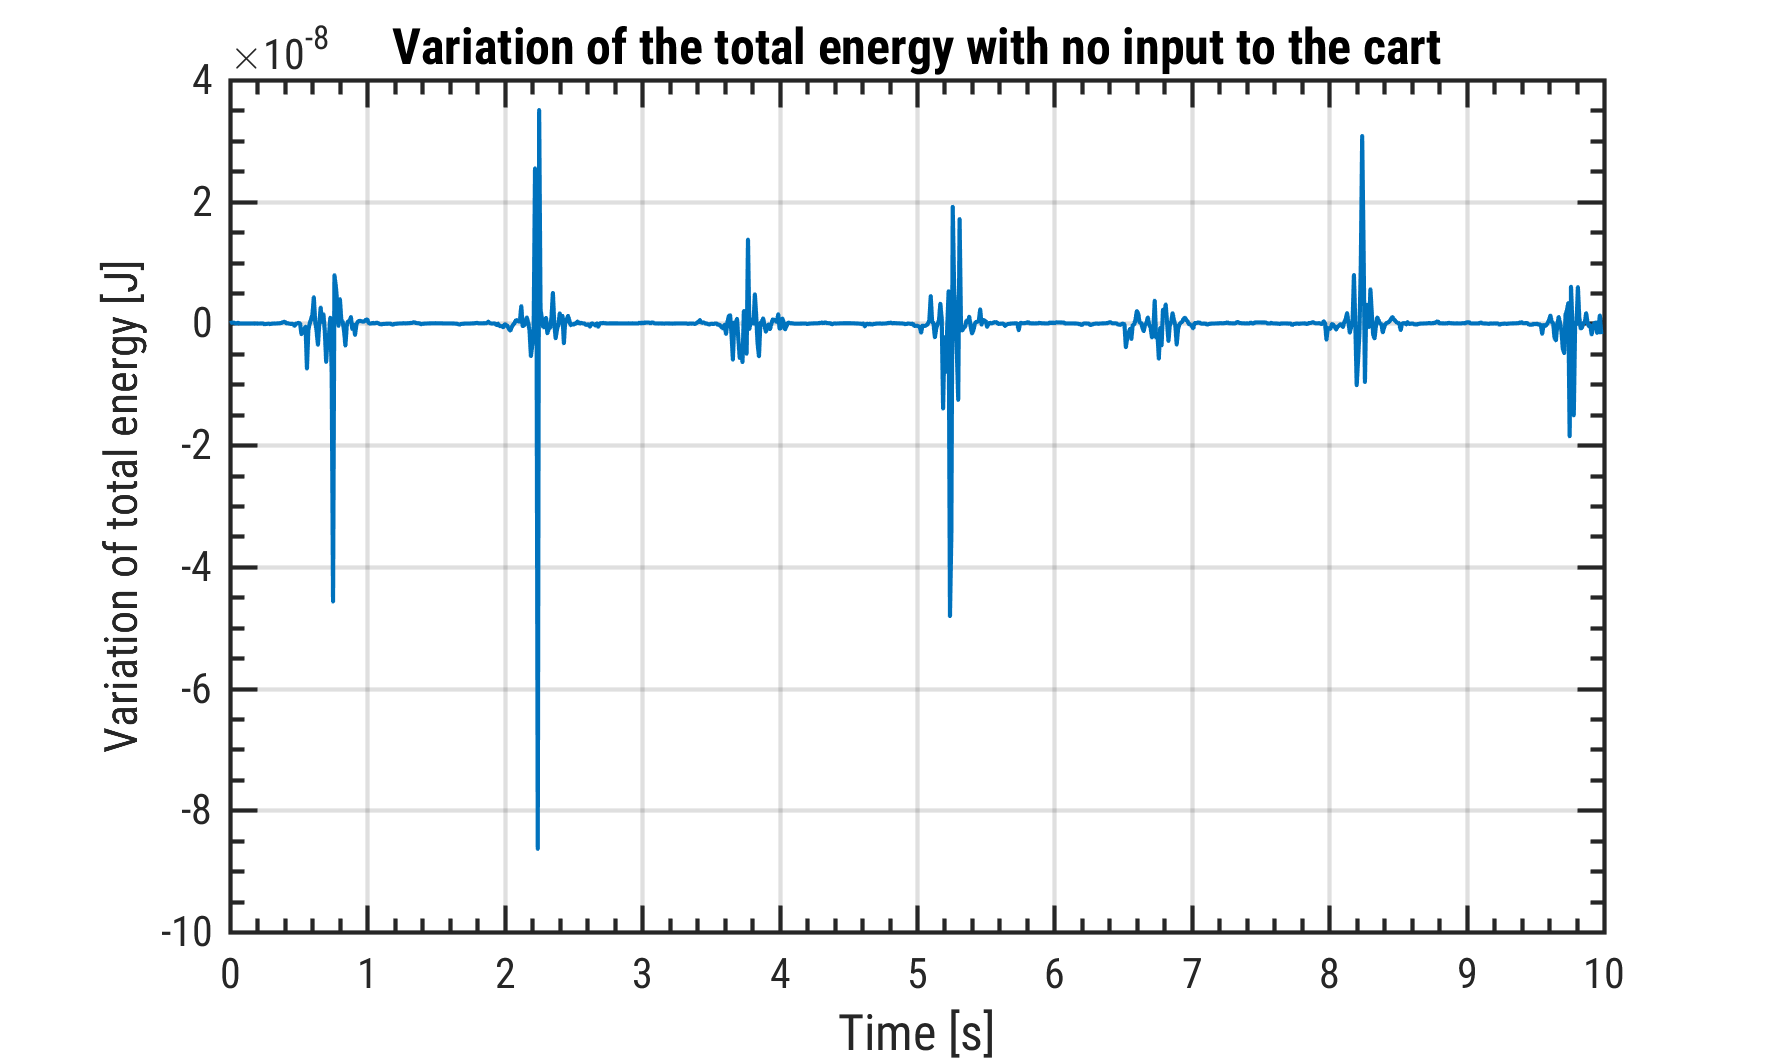
\includegraphics[width=16cm]{illustrations/check_model_variation.png}
	\caption{Variation of the total energy with no external forces on the cart with initial conditions $\mathbf{z}= [0,0,-\pi/2,0,-\pi/2,0,-\pi/2,0]^\text{T}$ simulated on MATLAB.}
	\label{fig:checkmodel_var}
\end{figure}

%---------------------------------------------------------------
%	IMPLEMENTATION OF THE LQR STABILIZATION
%---------------------------------------------------------------
\section{LQR controller}
\subsection{Brief overview of theory}
The main focus of the LQR controller is to handle both the limitation of the control signal $u$ and a fast transient phase for the system. A general block diagram of an LQR regulation is shown in \autoref{fig:block_dia_LQR}. It relies on minimizing a quadratic cost function $J$ which contains the states $\mathbf{z}$ and input $u$. In other words, the optimal regulation is likely to find a control input $u_1(t)$, $t\in[0,\infty[$ to the system dynamics in continuous time 
\[\dot{\mathbf{z}}=\mathbf{A}\,\mathbf{z}+\mathbf{B}\,u_1\]
that minimizes the cost function:
\[
J = \int^\infty_0 \left( z^T\mathbf{Q}z + u_1 R u_1 \right)\, \text{d}t
\]
where $\mathbf{Q}\in \mathbb{R}^{8\times8}$ is as a symmetric and positive-definite matrix weighting the states, and $R>0$ is a scalar weighting factor since $u_1$ is also a scalar. The feedback control law minimizing the value of $J$ is
\[u_1 = -\mathbf{K}\,\mathbf{z}\]
where $\mathbf{K}$ is given by $K=r^{-1}\,\mathbf{B}^T\mathbf{P}$. The matrix $\mathbf{P}$ is computed by solving the continuous time \emph{Riccati} equation
\[
\mathbf{A}^T\mathbf{P} + \mathbf{P\,A} - \mathbf{P\,B\,B}^T \mathbf{P}\,R^{-1} + \mathbf{Q} = 0
\]

The command \texttt{[K,P,E]=lqr(A,B,Q,R)} from MATLAB solves the Riccati equation and finds the optimal matrix gain $\mathbf{K}$.
\begin{figure}[h]
	\centering
	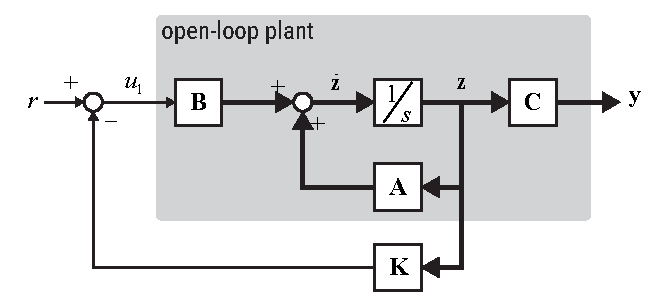
\includegraphics[width=13cm]{illustrations/block_dia_LQR.pdf}
	\caption{Block diagram of an LQR control system type with full state feedback}
	\label{fig:block_dia_LQR}
\end{figure}

\subsection{Controllability}
The satisfaction of the controllability property is crucial for designing a controller such as the LQR. It means that there exists a finite control input $u_1$ that the states of the system can be brought at any desired values $\mathbf{z}(t)$ from any initial values $\mathbf{z}_0$. For a system to be controllable, the rank of the controllability matrix $\mathcal{C}\in\mathbb{R}^{n\times n}$ must be equal to the number $n$ of state variable of the system ($n=8$ in the case of the triple pendulum).
\[ \text{rank}\left(\mathcal{C}\right) = \text{rank}\Big(\left[ \mathbf{B|AB|A}^2\mathbf{B}|\cdots|\mathbf{A}^{n-1}\mathbf{B} \right]\Big) =n \]
The controllability matrix can be computed using the MATLAB function \texttt{Co=ctrb(A,B)}. Concerning the rank of the controllability matrix, it can be found by using the function \texttt{n=rank(Co)}. One can also compute its singular value decomposition and count the number of nonzero values in order to check the controllability of the system.

%---------------------------------------------------------------
%	SWING-UP OF THE TRIPLE PENDULUM
%---------------------------------------------------------------
\section{Proposed control strategy}
The strategy chosen for the swing-up maneuver is based on reproducing the exact reversed behaviour of a falling triple pendulum.

\subsection{Generation of a downward trajectory} \label{sec:down_trajectory}
The necessary step of the swing-up maneuver is the planning of a motion that has to be followed. The trajectory is generated by recording the variation of the generalized coordinates during a falling of the triple pendulum. Before the record begins, the pendulum is placed in the configuration desired at the end of the swing-up maneuver. 

Since there is no friction in the pendulum, a proportional derivative controller is implemented to the cart. \autoref{fig:block_PD_cart} shows the implementation of the PD controller in the system. This controller will act as a spring and a damping component in order to dissipate the initial potential energy given by the upward initial configuration. The parameters of the PD controller and the initial configuration of the system are tuned such as during the falling, each link does not rotate several times on itself. With trial and error procedure, an ideal trajectory is found with appropriate parameters for the PD controller ($k_p=\num{0.3}\text{ and } k_i=\num{6.5}$) and the initial configuration ($\mathbf{z} = [0,0,0,\num{-0.4},0,\num{-0.6},0,\num{-0.6}]^\text{T}$). At the end of the generation of a trajectory, the history of variations of the generalized coordinates and the force applied on the cart by the controller are saved. They will be used for the swing-up maneuver.
\begin{figure}[ht]
	\centering
	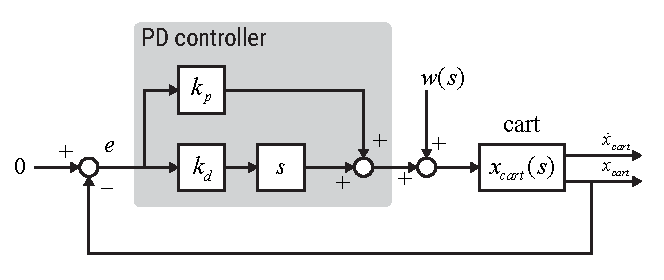
\includegraphics[width=15cm]{illustrations/block_PD_cart.pdf}
	\caption{Block diagram of the implementation of the PD controller in the triple pendulum. The $w(s)$ disturbance comes from the influences from the links to the cart.}
	\label{fig:block_PD_cart}
\end{figure}

\subsection{Swing-up maneuver with exact initial conditions}
As a first approach of the swing-up maneuver, the time-reversed input recorded is only provided as an input to the triple pendulum. Also the initial condition for the swing-up phase is equal to the last configuration $N$ recorded with reversed speeds.
\[
\mathbf{z}_{0,swing-up} = \big[ x_{cart_N},\, -\dot x_{cart_N} , \theta_{1_{N}},\, -\dot\theta_{1_{N}},\, \theta_{2_{N}},\, -\dot\theta_{2_{N}},\, \theta_{3_{N}},\, -\dot\theta_{3_{N}},\,  \big]^T
\]
At the end of this swing-up, the triple pendulum should have the same configuration as the one at the begining of the recorded trajectories.
\[
\mathbf{z}_{N,swing-up} = \big[ x_{cart_0},\, -\dot x_{cart_0} , \theta_{1_{0}},\, -\dot\theta_{1_{0}},\, \theta_{2_{0}},\, -\dot\theta_{2_{0}},\, \theta_{3_{0}},\, -\dot\theta_{3_{0}},\,  \big]^T
\]

\subsection{Swing-up maneuver with different initial conditions}
As the triple pendulum exhibits a hyperchaotic behaviour, a slight variation of initial conditions for the swing-up phase can lead to another complete configuration at the end of the swing-up maneuver. An idea is to reduce the initial deviation during the first seconds so that it is possible to catch the planned motion. To solve this issue, the implementation of an LQR is considered in order to fulfil the task.

The operating point of the LQR controller is set at the stable equlibrium ($\mathbf{z}_{eq}=[0\;0\;0\;0\;0\;0\;0\;0]^T$) of the triple pendulum. 


%\subsection{Stabilization}

%---------------------------------------------------------------
%	RESULTS
%---------------------------------------------------------------
% \newpage
\section{Numerical results}
\subsection{Generation of trajectories}
A trajectory is generated by setting the initial condition found in \autoref{sec:down_trajectory} and the mathematical model as input data to the function \texttt{ode45} from MATLAB. The duration of the simulation is set to $T=\SI{15}{\second}$ when the triple pendulum is nearly at rest. The results of the simulation are shown in \autoref{fig:result_gene}.

\begin{figure}[h]
    \centering
    \begin{subfigure}[t]{0.46\textwidth}
        \centering
        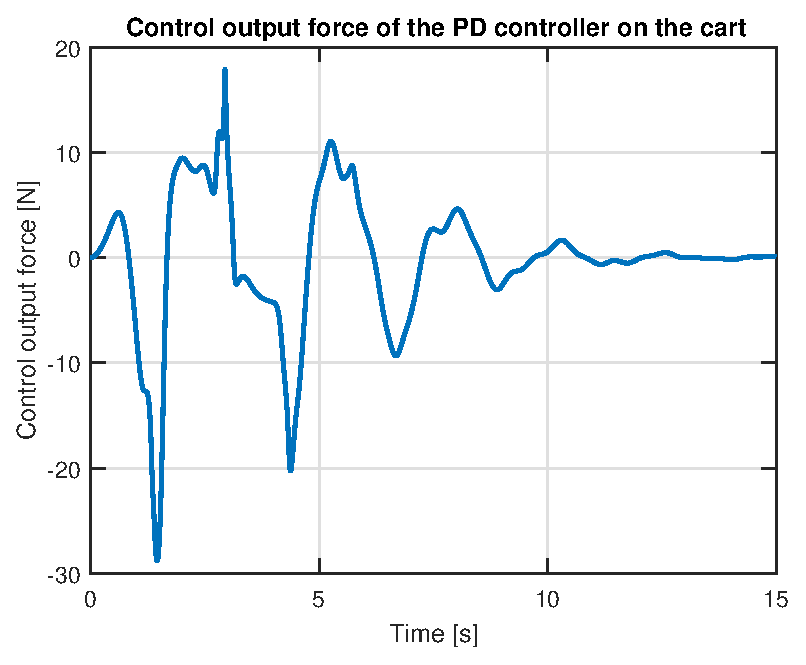
\includegraphics[width=1\textwidth]{graph_output_motion_plan}
        \caption{Output force of the PD controller}
    \end{subfigure}%
    ~ 
    \begin{subfigure}[t]{0.46\textwidth}
        \centering
        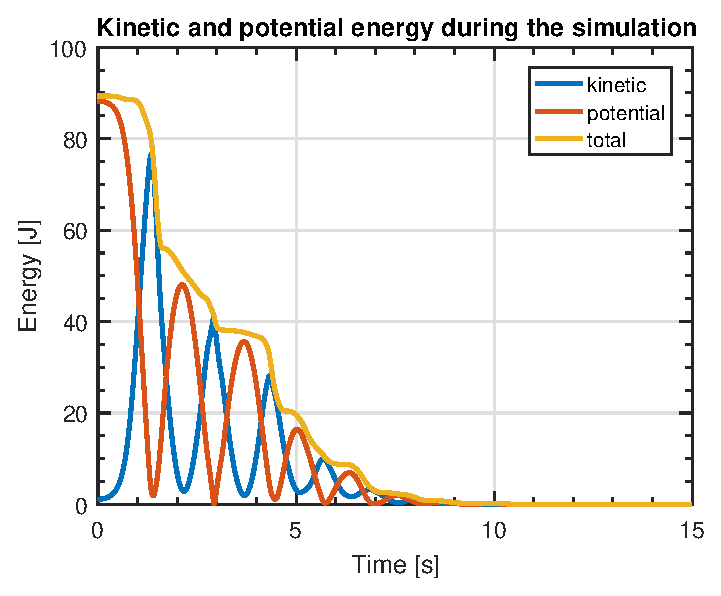
\includegraphics[width=1\textwidth]{graph_kineticpotential_energy_PD}
        \caption{Kinetic and potential energy}
    \end{subfigure}

    \begin{subfigure}[t]{0.46\textwidth}
        \centering
        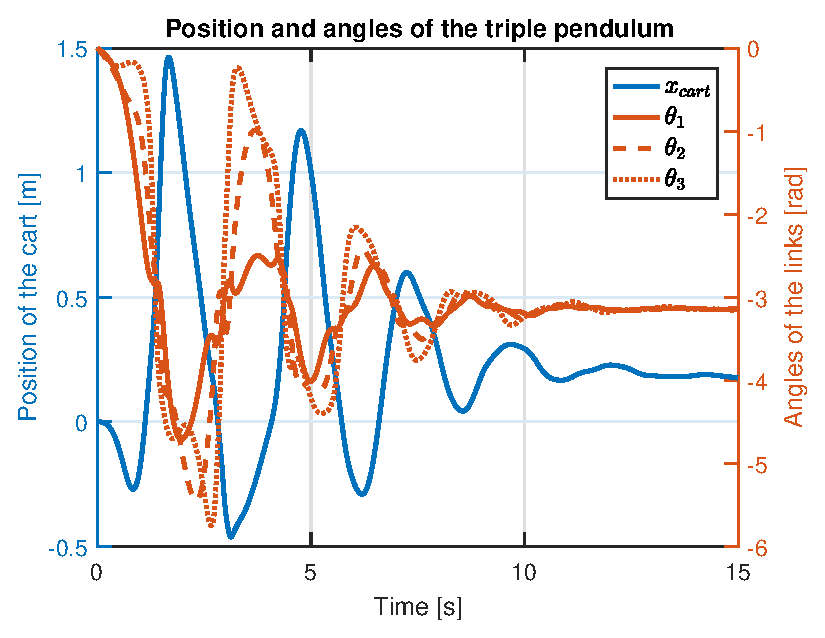
\includegraphics[width=1\textwidth]{graph_posangl_motion_plan}
        \caption{Position of cart and angles of links}
    \end{subfigure}%
    ~
    \begin{subfigure}[t]{0.46\textwidth}
        \centering
        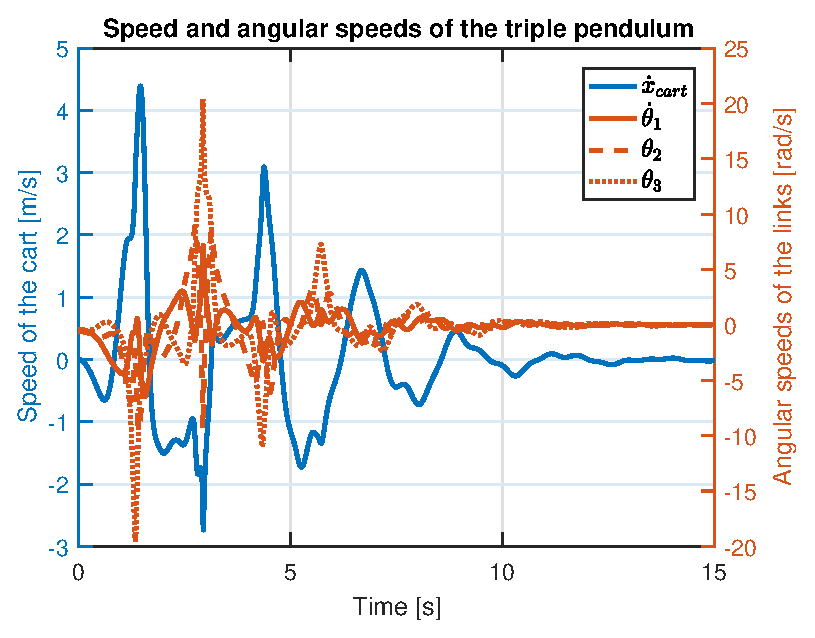
\includegraphics[width=1\textwidth]{graph_speed_motion_plan}
        \caption{Speed and angular speed}
    \end{subfigure}
    \caption{Simulation of a falling triple pendulum with initial conditions $\mathbf{z} = [0,0,0,\num{-0.4},0,\num{-0.6},0,\num{-0.6}]^\text{T}$}
     \label{fig:result_gene}
\end{figure}

\subsection{Swing-up maneuver simulation}
\paragraph{Exact initial conditions}
It is observed in \autoref{fig:actualvsplannedinit} that even the exact initial conditions are provided for the swing-up maneuver, there is a deviation at the end of the phase.
\begin{figure}[H]
    \centering
    \begin{subfigure}[h]{0.48\textwidth}
        \centering
        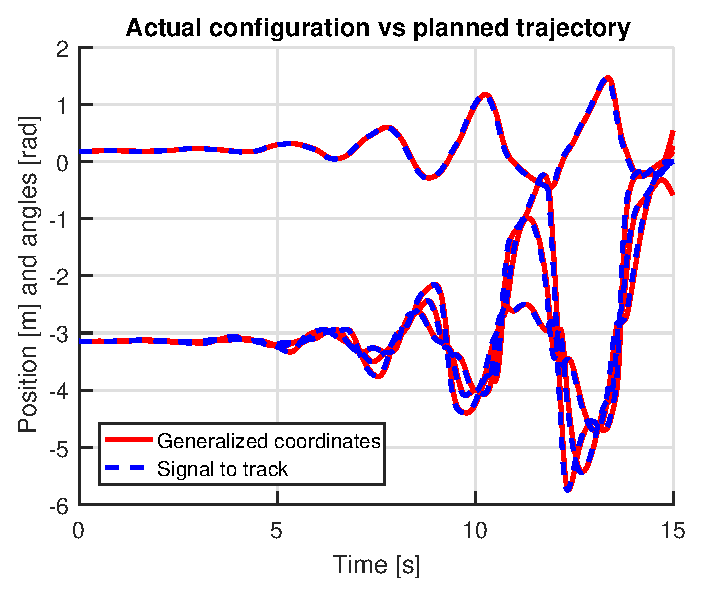
\includegraphics[width=1\textwidth]{illustrations/graph_swingup_pos_init.eps}
        \caption{Position and angles}
    \end{subfigure}%
    ~ 
    \begin{subfigure}[h]{0.48\textwidth}
        \centering
        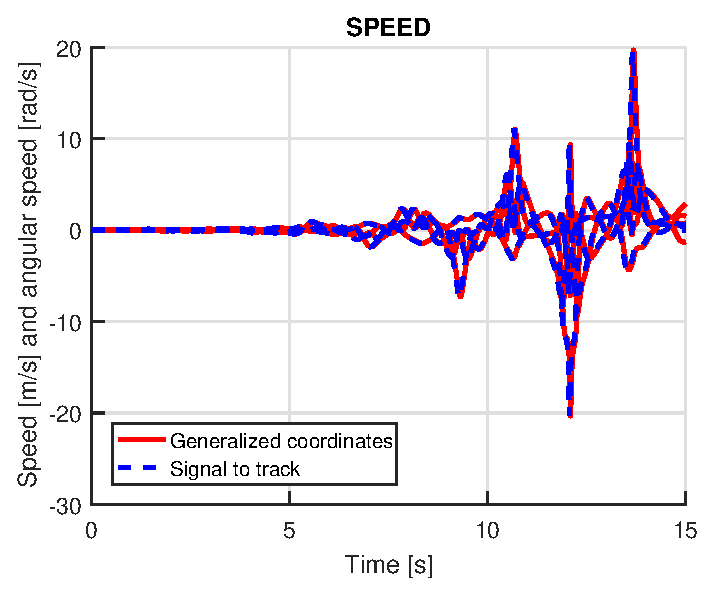
\includegraphics[width=1\textwidth]{illustrations/graph_swingup_speed_init.eps}
        \caption{Speed and angular speed}
    \end{subfigure}
    \caption{Actual vs planned trajectory}
    \label{fig:actualvsplannedinit}
\end{figure}

One can mesure the influence of the gap between the modified and planned initial conditions, a criterion is defined:
\[\Delta_{k,error}(t) = \big(z_k(t)-z_{k,planned}(t)\big)^2\]
The trajectory resulted from modified initial conditions (by adding \SI{0.1}{\radian} at every angles of the links) differs completely from the planned trajectory. This can be observed in \autoref{fig:compareerrormodinit}.
\begin{figure}[H]
    \centering
    \begin{subfigure}[h]{0.48\textwidth}
        \centering
        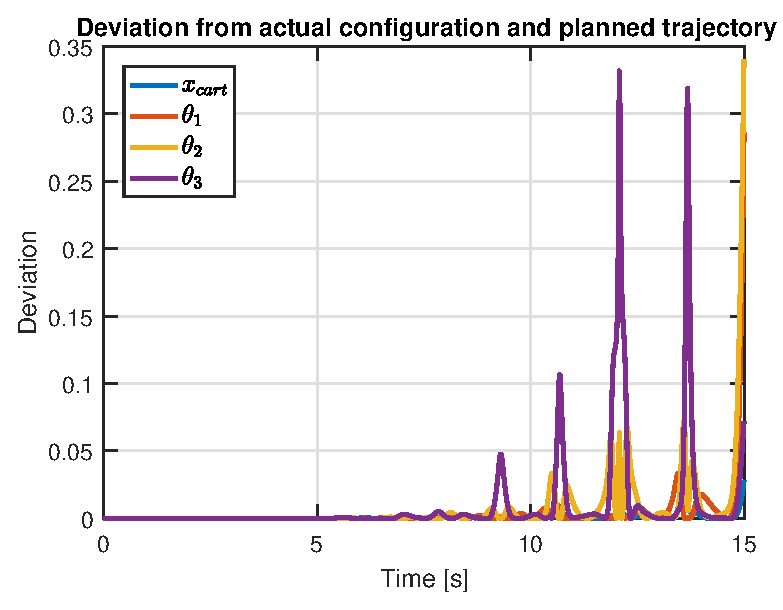
\includegraphics[width=1\textwidth]{illustrations/graph_error_init.eps}
        \caption{Exact initial conditions}
    \end{subfigure}%
    ~ 
    \begin{subfigure}[h]{0.48\textwidth}
        \centering
        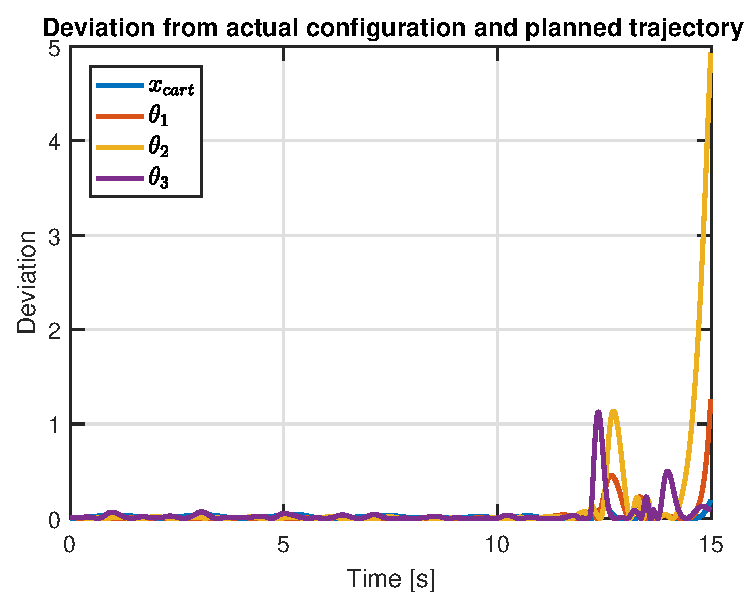
\includegraphics[width=1\textwidth]{illustrations/graph_error_mod.eps}
        \caption{Modified initial conditions}
    \end{subfigure}
    \caption{Comparison between trajectories with exact and modified initial conditions. The modified initial conditions are changed by adding \SI{0.1}{\radian} for all angles of the link.}
    \label{fig:compareerrormodinit}
\end{figure}

\paragraph{Different initial conditions}
In order to handle initial conditions different from the planned trajectory, an LQR is applied for the first 10 seconds. The linearized state-space model is done around $\mathbf{z}_{LQR}=[0,\,0,\,-\pi,\, 0,\, -\pi,\,0,\,-\pi,\,0]^T$. Thus the matrices $\mathbf{A}$ and $\mathbf{B}$ obtained are:
\begin{equation}
\mathbf{A} = 
\begin{bmatrix}
 0 & 1 &        0 & 0 &        0 &      0 &        0 &      0 \\
 0 & 0 &  24.1343 & 0 &  -3.9493 &      0 &   0.4388 &      0 \\
 0 & 0 &        0 & 1 &        0 &      0 &        0 &      0 \\
 0 & 0 & -70.2090 &      0 &  35.5433 &      0 &  -3.9493 &      0 \\
 0 & 0 &        0 &      0 &        0 & 1 &        0 &      0 \\
 0 & 0 &  59.2388 &      0 & -65.8209 &      0 &  17.1134 &      0 \\
 0 & 0 &        0 &      0 &        0 &      0 &        0 & 1 \\
 0 & 0 & -19.7463 &      0 &  51.3403 &      0 & -35.1045 &      0 \\
\end{bmatrix},\quad
\mathbf{B} =
\begin{bmatrix}
     0\\
0.7761\\
     0\\
-0.9851\\
     0\\
0.2687\\
     0\\
-0.0896\\
\end{bmatrix}.
\end{equation}
The controllability condition is verified since $\text{rank}(\mathcal{C})=8$.
Since there is no guideline for selecting the weighting coefficient $\mathbf{Q}$ and $R$, an adequate choice found is
\begin{equation}
\begin{split}
\mathbf{Q}&=\text{diag}\big(100\quad0\quad100\quad0\quad100\quad0\quad100\quad0\big)\\
R&=0.5
\end{split}
\end{equation}
The resulted gain matrix is given by
\begin{equation}
\mathbf{K}=\big[14.1421\quad12.6550\quad-18.0235\quad2.6144\quad-0.0900\quad1.2742\quad1.8248\quad0.3713\big]
\end{equation}
With initial conditions modified by adding \SI{0.1}{\radian} at each angle, the deviation in function of time is plotted in \autoref{fig:error_LQR}. One can observe that for the first 3 seconds, the LQR regulator achieves to catch up the planned trajectory.
\begin{figure}[h]
	\centering
	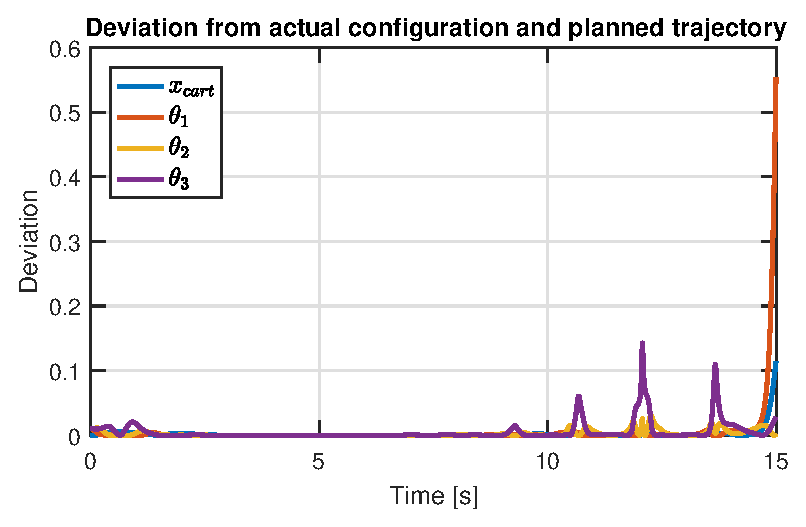
\includegraphics[width=12cm]{illustrations/graph_error_LQR.eps}
	\caption{Deviation from actual configuration and planned trajectory. The offset added to initial conditions is $\mathbf{z}_{0,offset}=[0,0,0.1,0,0.1,0,0.1,0]^T$.}
	\label{fig:error_LQR}
\end{figure}

The sum of errors for each simulation are resumed in \autoref{tab:performance}
\begin{table}[H]
\centering
\caption{Performance for each simulation}
\label{tab:performance}
\begin{tabular}{|l|l|l|l|}
\hline
Initial conditions                       & Exact & Modified & Modified with LQR \\ \hline
Sum of errors between actual and planned & 31.44 & 333.88   & 22.26             \\ \hline
\end{tabular}
\end{table}
\newpage
%---------------------------------------------------------------
%	CONCLUSION
%---------------------------------------------------------------
\section{Conclusion and recommendations}
In the light of the above, the time-reversal strategy provides an interesting method for the swing-up of the triple pendulum. The forces involved for the swing-up maneuver is limited. This can be suitable for systems which requires smooth accelerations. However the time needed for the pendulum to switch to the up equilibrium is equal to the time needed for the pendulum to fall and stabilize. It is much more longer than other methods such as the one treated by \citet{Gluck2013801}. In their case, they achieved a transition time of \SI{3.5}{\second}.

One downfall of this method is that the generation of a trajectory is not done in an automatically way. Any changes in the pendulum parameters require to adapt the initial conditions for the generation of an ideal trajectory. Also period for which the LQR regulator is applied is set manually according to the behaviour of the pendulum. A trial and error method is required for an ideal trajectory.

The swing-up maneuver with exact initial conditions leads to a sgnificant deviation from the generated trajectory at the end of the phase. It should normally be exactly at the upright configuration at the end of the swing-up phase. However it is not the case and this might be due to numerical errors from the ODE function.

The single LQR applied for long periods in order to cope the deviations from planned trajectory is not adapted for this strategy. Indeed, since it is designed around an operating configuration, the linearized state-space model can not be correct during the first seconds. One mean of improvement is to design several LQRs along the trajectory with the purpose that several linearized state-space models along the time can approach the non-linear behaviour.

%---------------------------------------------------------------
%	APPENDIX
%---------------------------------------------------------------
\newpage
\appendix
\section{MATLAB scripts and function files}
\begin{description}
	\item[File:] \texttt{math\_model\_pendulum.m}
	\item[Description:] Derivating the mathematical model of the triple pendulum using the symbolic math toolbox from MATLAB. It returns the expressions of the second order derivative of generalized coordinates.
\end{description}
\begin{lstlisting}[label=code:mathmodelpendulum,caption=\texttt{math\_model\_pendulum.m}]
syms M m1 m2 m3;
syms x xd xdd theta1 theta1d theta1dd theta2 theta2d theta2dd theta3 theta3d theta3dd;
syms l1 l2 l3;
syms u1 u2 u3 u4;
syms g;

%%%%%%%%%%%%%%%%%%% POSITION OF CENTER OF MASS %%%%%%%%%%%%%%%%%%%%%%%%%%%%
p1 = [x - l1/2*sin(theta1); l1/2*cos(theta1)];
p2 = [x - l1*sin(theta1) - l2/2*sin(theta2); l1*cos(theta1) + l2/2*cos(theta2)];
p3 = [x - l1*sin(theta1) - l2*sin(theta2) - l3/2*sin(theta3); l1*cos(theta1) + l2*cos(theta2) + l3/2*cos(theta3)];

%%%%%%%%%%%%%%%%%%%%% SPEED OF CENTER OF MASS%%%%%%%%%%%%%%%%%%%%%%%%%%%%%%
p1d = diff(p1,x)*xd + diff(p1,theta1)*theta1d;
p2d = diff(p2,x)*xd + diff(p2,theta1)*theta1d + diff(p2,theta2)*theta2d;
p3d = diff(p3,x)*xd + diff(p3,theta1)*theta1d + diff(p3,theta2)*theta2d + diff(p3,theta3)*theta3d;

%%%%%%%%%%%%%%%%%% LAGRANGIAN OF THE TRIPLE PENDULUM %%%%%%%%%%%%%%%%%%%%%%
% Kinetic energy
KE = 0.5 * (M*xd^2 + m1*(p1d.')*p1d + m2*(p2d.')*p2d + m3*(p3d.')*p3d) + ...
    0.5 * (m1*l1^2/12*theta1d^2 + m2*l2^2/12*theta2d^2 + m3*l3^2/12*theta3d^2);
KE = simplify(KE);

% Potential energy
PE = g * (m1*p1(2) + m2*p2(2) + m3*p3(2));

% Lagrangian derivation
KExd = diff(KE,xd);
dtKExd = diff(KExd,xd)*xdd + ...
	diff(KExd,theta1)*theta1d + diff(KExd,theta1d)*theta1dd + ...
	diff(KExd,theta2)*theta2d + diff(KExd,theta2d)*theta2dd + ...
	diff(KExd,theta3)*theta3d + diff(KExd,theta3d)*theta3dd;
KEx = diff(KE,x);
PEx = diff(PE,x);

KEtheta1d = diff(KE,theta1d);
dtKEtheta1d = diff(KEtheta1d,theta1)*theta1d + diff(KEtheta1d,theta1d)*theta1dd + ...
	diff(KEtheta1d,xd)*xdd + ...
	diff(KEtheta1d,theta2)*theta2d + diff(KEtheta1d,theta2d)*theta2dd + ...
	diff(KEtheta1d,theta3)*theta3d + diff(KEtheta1d,theta3d)*theta3dd;
KEtheta1 = diff(KE,theta1);
PEtheta1 = diff(PE,theta1);

KEtheta2d = diff(KE,theta2d);
dtKEtheta2d = diff(KEtheta2d,theta1)*theta1d + diff(KEtheta2d,theta1d)*theta1dd + ...
	diff(KEtheta2d,xd)*xdd + ...
	diff(KEtheta2d,theta2)*theta2d + diff(KEtheta2d,theta2d)*theta2dd + ...
	diff(KEtheta2d,theta3)*theta3d + diff(KEtheta2d,theta3d)*theta3dd;;
KEtheta2 = diff(KE,theta2);
PEtheta2 = diff(PE,theta2);

KEtheta3d = diff(KE,theta3d);
dtKEtheta3d = diff(KEtheta3d,theta1)*theta1d + diff(KEtheta3d,theta1d)*theta1dd + ...
	diff(KEtheta3d,xd)*xdd + ...
	diff(KEtheta3d,theta2)*theta2d + diff(KEtheta3d,theta2d)*theta2dd + ...
	diff(KEtheta3d,theta3)*theta3d + diff(KEtheta3d,theta3d)*theta3dd;
KEtheta3 = diff(KE,theta3);
PEtheta3 = diff(PE,theta3);

%%%%%%%%%%%%%%%%%%%%%%%% EQUATIONS OF MOTION %%%%%%%%%%%%%%%%%%%%%%%%%%%%%%
eqx1 = simplify(dtKExd - KEx + PEx - u1);
eqx2 = simplify(dtKEtheta1d - KEtheta1 + PEtheta1);
eqx3 = simplify(dtKEtheta2d - KEtheta2 + PEtheta2);
eqx4 = simplify(dtKEtheta3d - KEtheta3 + PEtheta3);

Sol = solve(eqx1,eqx2,eqx3,eqx4,xdd,theta1dd,theta2dd,theta3dd)

syms z1 z2 z3 z4 z5 z6 z7 z8;
fx1 = subs(Sol.xdd, {x,xd,theta1,theta1d,theta2,theta2d,theta3,theta3d}, {z1,z2,z3,z4,z5,z6,z7,z8});
fx2 = subs(Sol.theta1dd, {x,xd,theta1,theta1d,theta2,theta2d,theta3,theta3d}, {z1,z2,z3,z4,z5,z6,z7,z8});
fx3 = subs(Sol.theta2dd, {x,xd,theta1,theta1d,theta2,theta2d,theta3,theta3d}, {z1,z2,z3,z4,z5,z6,z7,z8});
fx4 = subs(Sol.theta3dd, {x,xd,theta1,theta1d,theta2,theta2d,theta3,theta3d}, {z1,z2,z3,z4,z5,z6,z7,z8});

fx1 = simplify(fx1);
fx2 = simplify(fx2);
fx3 = simplify(fx3);
fx4 = simplify(fx4);

fx = [fx1 fx2 fx3 fx4];
\end{lstlisting}

\begin{description}
	\item[File:] \texttt{math\_model\_linear.m}
	\item[Description:] Symbolic computation of the linearized state-space model by using the mathematical model from \texttt{math\_model\_pendulum.m}. Returns the expressions of jacobian matrices $\mathbf{A}$ and $\mathbf{B}$.
\end{description}
\begin{lstlisting}[label=code:mathmodellinear,caption=\texttt{math\_model\_linear.m}]
syms u1 z1 z2 z3 z4 z5 z6 z7 z8;
feq1 = z2;
feq2 = subs(fx1, {x,xd,theta1,theta1d,theta2,theta2d,theta3,theta3d}, {z1,z2,z3,z4,z5,z6,z7,z8});
feq3 = z4;
feq4 = subs(fx2, {x,xd,theta1,theta1d,theta2,theta2d,theta3,theta3d}, {z1,z2,z3,z4,z5,z6,z7,z8});
feq5 = z6;
feq6 = subs(fx3, {x,xd,theta1,theta1d,theta2,theta2d,theta3,theta3d}, {z1,z2,z3,z4,z5,z6,z7,z8});
feq7 = z8;
feq8 = subs(fx4, {x,xd,theta1,theta1d,theta2,theta2d,theta3,theta3d}, {z1,z2,z3,z4,z5,z6,z7,z8});

A = jacobian([feq1; feq2; feq3; feq4; feq5; feq6; feq7; feq8], [z1 z2 z3 z4 z5 z6 z7 z8]);
B = jacobian([feq1; feq2; feq3; feq4; feq5; feq6; feq7; feq8], u1);

save('state_space_symb.mat','A','B')
\end{lstlisting}

\begin{description}
	\item[File:] \texttt{LQR\_controller.m}
	\item[Description:] The function verifies if the system is controllable at a certain operating configuration $\mathbf{z}$ and returns the gain matrix $\mathbf{K}$. It uses the expressions of $\mathbf{A}$ and $\mathbf{B}$ from \texttt{math\_model\_linear.m} in order to find the linearized state-space model.
\end{description}
\begin{lstlisting}[label=code:LQR,caption=\texttt{LQR\_controller.m}]
function K=LQR_controller(z,u)
  %%%%%%%% LINEARIZATION OF THE SYSTEM %%%%%%%%
  % Loading state-space model and parameters
  load('state_space_symb.mat')
  l1 = 1;     l2 = 1;     l3 = 1;  % length of the links
  m1 = 1;     m2 = 1;     m3 = 1;  % masses at the end of each link
  M  = 1;                          % mass of the cart
  g  = 9.8;
  u1 = u;

  % Linearizing around the following configuration
  z1 = z(1); z2 = z(2);
  z3 = z(3); z4 = z(4);
  z5 = z(5); z6 = z(6);
  z7 = z(7); z8 = z(8);

  A_lin = eval(A);
  B_lin = eval(B);

  C = zeros(4,8);
  C(1,1) = 1;
  C(2,3) = 1;
  C(3,5) = 1;
  C(4,7) = 1;
  D = 0;

  %%%%%%%%%%%%%%% CONTROLABILITY OF THE LINEARIZED SYSTEM %%%%%%%%%%%%%%%
  Co = ctrb(A_lin,B_lin);
  r_Co = rank(Co);

  if r_Co == 8
    fprintf('The system is controllable. Rank of Co: %d \n',r_Co);
  else
    fprintf('The system is not controllable. Rank of Co: %d \n',r_Co);
  end

  %%%%%%%%%%%%%%%%%% LQR CONTROLLER %%%%%%%%%%%%%%%%%%
  R = 1;
  Q = C'*C;
  Q = diag([1 0 1 0 1 0 1 0]);

  [K,P,E] = lqr(A_lin,B_lin,Q,R);
end
\end{lstlisting}

\begin{description}
	\item[File:] \texttt{sim\_generate\_motion.m}
	\item[Description:] This script simulates a falling triple pendulum with initial conditions \texttt{z0} in order to generate a trajectory. It calls the function \texttt{triple\_pendulum\_ODE.m} which defines the system of differential equations.
\end{description}
\begin{lstlisting}[label=code:simgenerate,caption=\texttt{sim\_generate\_motion.m}]
%%%%%%%%% DEFINITIONS OF THE PARAMETERS %%%%%%%%%
k1 = 0.3;   k2 = 6.5;           % constants for the PD controller
param = struct('l1',1,'l2',1,'l3',1, ...        % length of the links
        'm1',1,'m2',1,'m3',1,'M',1,....   % masses
        'g',9.8);
u=0;

%%%%% SETTING PARAMETERS FOR THE ODE SOLVER %%%%%
init_t = 0;
final_t = 15;
dt = 0.01;
N = (final_t-init_t)/dt;
t_span = init_t:dt:final_t-dt;

%%%%%%%%%%%%% INITIAL CONDITIONS %%%%%%%%%%%%%%%%
z0 = [0 0 0 -0.4 0 -0.6 0 -0.6]';

zhistory1 = zeros(N,8);
uhistory1 = zeros(N,1);
t_history = zeros(N,1);

%%%%%%%%%%%%%%%%%% ODE SOLVER %%%%%%%%%%%%%%%%%%%
options = odeset('abstol',1e-9,'reltol',1e-9);

zprec = z0;
u = 0;

for i =1:N
    clc
    fprintf('%d / %d',i,N);
    [t1,z1] = ode113(@triple_pendulum_ODE, [0 dt 0.2], ...
        zprec,options,u,param);
    u = -k1*z1(2,1)-k2*z1(2,2);
    uhistory1(i) = u;
    t_history(i) = t1(2);
    zhistory1(i,:) = z1(2,:);
    zprec = z1(2,:);
    if z1(2,1)>=4 || z1(2,1)<=-4
        fprintf('ODE113 terminated, out of bounds');
        break
    end
end
u0 = 0;
zhistory1 = [z0'; zhistory1];
zhistory1(end,:) = [ ];

save('trajectory_history.mat','zhistory1','uhistory1','t_history')
\end{lstlisting}

\begin{description}
	\item[File:] \texttt{triple\_pendulum\_ODE.m}
	\item[Description:] MATLAB function defining the system of differential equations. The dynamics were derived in \autoref{equ:model_final} and from \texttt{math\_model\_pendulum.m}. \emph{Note:} lines 24, 26 28 and 30 are shown partially in \autoref{code:tripleODE}.
\end{description}
\begin{lstlisting}[label=code:tripleODE,caption=\texttt{triple\_pendulum\_ODE.m}]
function dz = triple_pendulum_ODE(t,z,u,param)
    load('motion_equations.mat','fx');
	z1 = z(1);
	z2 = z(2);
	z3 = z(3);
	z4 = z(4);
	z5 = z(5);
	z6 = z(6);
	z7 = z(7);
	z8 = z(8);
	u1 = u;

  	l1 = param.l1;
  	l2 = param.l2;
  	l3 = param.l3;
  	m1 = param.m1;
  	m2 = param.m2;
  	m3 = param.m3;
  	M  = param.M;
  	g  = param.g;

  	% These equations are derived from the file Symb_Development_3DOF
	dz1 = z2;
	dz2 = -(144*m2^2*u1*cos(2*z3 - 2*z5) - 144*m3^2*u1 - 240*m2^2*u1 + [...]
	dz3 = z4;
	dz4 = -(24*(6*m2^2*u1*cos(z3 - 2*z5) - 6*m3^2*u1*cos(z3) - 4*g*m2^3*sin(z3) - [...]
	dz5 = z6;
	dz6 = (24*(12*m2^2*u1*cos(z5) - 6*m3^2*u1*cos(2*z3 - z5) - 12*m2^2*u1*cos(2*z3 - z5) + [...]
	dz7 = z8;
	dz8 = (36*m2^2*u1*cos(2*z3 - z7) - 108*m2^2*u1*cos(2*z5 - z7) - 36*m2^2*u1*cos(z7) + [...]

	dz = [dz1 dz2 dz3 dz4 dz5 dz6 dz7 dz8]';
\end{lstlisting}

\begin{description}
	\item[File:] \texttt{sim\_swingup\_motion.m}
	\item[Description:] This MATLAB script simulates the swing-up maneuver of the triple pendulum. The initial conditions \texttt{z0} and also the control strategy can be changed.
\end{description}
\begin{lstlisting}[label=code:simswingup,caption=\texttt{sim\_swingup\_motion.m}]
%%%%%%%%% DEFINITIONS OF THE PARAMETERS %%%%%%%%%
param = struct('l1',1,'l2',1,'l3',1, ...        % length of the links
        'm1',1,'m2',1,'m3',1,'M',1,....   % masses
        'g',9.8);
k1 = 0.5;   k2 = 4;              % constants for the PD controller
u = 0;

load('trajectory_history.mat')

%%%%% SETTING PARAMETERS FOR THE ODE SOLVER %%%%%
init_t = 0;
final_t = 15;
dt = 0.01;
N = (final_t-init_t)/dt;
t_span = init_t:dt:final_t-dt;

%%%%%%%%%%%%% INITIAL CONDITIONS %%%%%%%%%%%%%%%%
zhistory2 = [];
uhistory = [];

zhistory1_reversed = zeros(size(zhistory1));
uhistory1_reversed = zeros(size(uhistory1));
for i = 1:size(zhistory1_reversed,1)
    zhistory1_reversed(i,:) = zhistory1(end-i+1,:);
    uhistory1_reversed(i) = uhistory1(end-i+1);
end

zhistory1_reversed(:,2) = -zhistory1_reversed(:,2);
zhistory1_reversed(:,4) = -zhistory1_reversed(:,4);
zhistory1_reversed(:,6) = -zhistory1_reversed(:,6);
zhistory1_reversed(:,8) = -zhistory1_reversed(:,8);

x0 = zhistory1_reversed(1,:)' + [0;0;0.1;0;0.1;0;0.1;0]; % adding an offset to initial conditions

%%%%%%%%%%%%%%% LQR CONTROLLER  %%%%%%%%%%%%%%%%
x1 = [0 0 -pi 0 -pi 0 -pi 0]';
u1 = 0;
K1 = LQR_controller(x1,u1);

%%%%%%%%%%%%%%%%%% ODE SOLVER %%%%%%%%%%%%%%%%%%%
options = odeset('abstol',1e-9,'reltol',1e-9);
% [t,z] = ode113(@three_dof_arm_cart_dyn_for_ODE_up, t_span, x0, options,u,l1,l2,l3,m1,m2,m3,M,g);

xprec = x0;
for i =1:N
    clc;
    fprintf('%d / %d',i,N);
    [t1,z1] = ode45(@three_dof_arm_cart_dyn_for_ODE_up, [0 dt 0.05], xprec,options,u,param);
    zhistory2 = [zhistory2; z1(2,:)];
    if i<= 900
        u = -K1*(z1(2,:)-zhistory1_reversed(i,:))' + uhistory1_reversed(i);
    else
        u = uhistory1_reversed(i);
    end
    xprec = z1(2,:);
    if z1(2,1)>=4 || z1(2,1)<=-4
        fprintf('ODE113 terminated, out of bounds');
        break
    end
end

zhistory2 = [x0'; zhistory2];
zhistory2(end,:) = [ ];
\end{lstlisting}


\newpage
\addcontentsline{toc}{section}{References}
\nocite{*}
\bibliographystyle{plainnat}
\bibliography{bibliography}
\end{document}
